
\section{Stable Matching}

motivation: set up pairings between different entities, where each side has a notion of preference 

% \medskip

\begin{definition}[Matching]\label{def:matching}
Given a pair of sets $M$ and $W$, a matching \(S\) is a collection of pairs \((m,w)\), where \(m \in M\) and \(w \in W\), and each element from either set appears in at most one pair. 
A matching is perfect if no element remains unmatched.
\end{definition}

\begin{definition}[Stability]\label{def:stability}
Given sets $M$ and $W$ of equal size and a preference ordering for each element of each set, a stable matching is a perfect matching where no unstable pair exists.
An unstable pair is a pair \((m,w)\) that is \emph{not} in the matching such that \(m\) and \(w\) prefer each other to their current partners in the matching.
\end{definition}

given two sets \(M\) and \(W\) of equal size \(n\), where every \(m\in M\) and every \(w\in W\) has a strict and complete preference list over the elements of the other set
% \(2n\) strict and complete preference lists, each consisting of \(n\) elements (one list for every \(m\in M\) and every \(w\in W\)), where \(n = |M| = |W|\)

\begin{algorithm}[h]
\caption{Propose-and-Reject (Gale-Shapley, 1962)}
\label{alg:gale_shapley}
\begin{algorithmic}[1]
  \Require \(2n\) strict and complete preference lists, each consisting of \(n\) elements
  \Ensure a matching \(S^*\) that pairs each \(m\in M\) with each \(w\in W\)
  \State initialize all \(m\in M\) and \(w\in W\) as \attribute{free}
  \While{there exists a \attribute{free} \(m\in M\) who has not proposed to every \(w\in W\)}
    \State choose such an \(m\)
    \State \(w\) \(\gets\) highest ranked element on \(m\)'s list to whom \(m\) has not yet proposed
    \State \(m\) proposes to \(w\)
    \If{\(w\) is \attribute{free}}
      \State match \(m\) and \(w\)
    \ElsIf{\(w\) prefers \(m\) to her current partner \(m'\)}
      \State match \(m\) and \(w\)
      \State mark \(m'\) as \attribute{free}
    \Else
      \State \(w\) rejects \(m\)'s proposal
    \EndIf
  \EndWhile
  \State \Return \(S^*\)
\end{algorithmic}
\end{algorithm}


\begin{observation}\label{obs:gale_shapley:men_propose_in_decreasing_order}
\(M\) propose to \(W\) in decreasing order of preference.
\end{observation}

\begin{observation}\label{obs:gale_shapley:women_only_trade_up}
Once a \(w\in W\) is matched, it never becomes unmatched, it only trades up.
\end{observation}


\subsection{Correctness}

\begin{claim}[Correctness: Termination]
\label{clm:gale_shapley:termination}
\autoref{alg:gale_shapley} terminates after at most \(n^2\) iterations of the while-loop.
\end{claim}

\begin{proof}\label{proof:gale_shapley:termination}
\leavevmode
% \begin{itemize}[nolistsep, noitemsep]
% \item 
There is one proposal per iteration.
% \item 
By \autoref{obs:gale_shapley:men_propose_in_decreasing_order}, once a \(m\in M\) has proposed to a \(w\in W\), it never proposes to \(w\) again. 
So each \(m\in M\) does \(\leq n\) proposals.
% \item 
There are \(n\) elements in \(M\), and each does \(\leq n\) proposals. 
After \(\leq n^2\) iterations, no one is left to propose to. 
Thus, \autoref{alg:gale_shapley} must terminate after \(\leq n^2\) iterations.
% \qedhere
% \end{itemize}
\end{proof}


\begin{claim}[Correctness: Perfect Matching]\label{clm:gale_shapley:perfection}
Every \(m\in M\) and every \(w\in W\) gets matched by \autoref{alg:gale_shapley}.
\end{claim}

\begin{proof}[Contradiction]\label{proof:gale_shapley:perfection}
Assume there is a \(m\in M\) who is unmatched.
Since \(|M| = |W|\), there must also be a \(w\in W\) who is unmatched.
By \autoref{obs:gale_shapley:women_only_trade_up}, \(w\) was never proposed to.
But for \(m\) to remain unmatched after termination, \(m\) must have proposed to every \(w\in W\), including this \(w\).
\end{proof}


\begin{claim}[Correctness: Stability]\label{clm:gale_shapley:stability}
The matching created by \autoref{alg:gale_shapley} is stable.
\end{claim}

\begin{proof}[Contradiction]\label{proof:gale_shapley:stability}
Assume there is an unstable pair \((m, w)\), where \(m \in M\) and \(w \in W\) after termination of \autoref{alg:gale_shapley}.


\medskip

We can distinguish two cases:\tikzmark{distinguish-cases}%
\begin{tikzpicture}[>=latex, remember picture, overlay, scale=1]
\coordinate (distinguishcases-y) at (pic cs:distinguish-cases);
\coordinate (distinguishcases-border) at (current page.east |- distinguishcases-y);
\coordinate (distinguishcases-margin) at ($(distinguishcases-border) + 0.5*(\textwidth,0) + 0.5*(-\paperwidth,0)$);
\begin{scope}[shift={(distinguishcases-margin)}, scale=0.8]
\begin{scope}[shift={(-2,-0.75)}]
\def\matchingellipse{(0,0) ellipse (2 and 1)}
\filldraw[fill=gray!20, draw=gray!60]\matchingellipse;
\node[left] at (-1.6,0.8) {\footnotesize matching};
\node (m) at (-1.0,0.5) {\footnotesize $m$};
\node (w) at (1.0,0.5) {\footnotesize $w$};
\node (mp) at (-1.0,-0.5) {\footnotesize $m'$};
\node (wp) at (1.0,-0.5) {\footnotesize $w'$};
\draw[densely dotted, latex -latex] (m) -- node[pos=0.5, above]{\footnotesize ?} (w);
\draw[latex -latex] (m) -- (wp);
\draw[latex -latex] (mp) -- (w);
\end{scope}
\end{scope}
\end{tikzpicture}

\begin{enumerate}[label=Case \arabic*:, ref=Case \arabic*, leftmargin=*, labelindent=1em, itemsep=\smallskipamount, topsep=\medskipamount]
\item \(m\) never proposed to \(w\) \label{proof:gale_shapley:stability:case:never_proposed}
\item \(m\) proposed to \(w\) \label{proof:gale_shapley:stability:case:proposed}
\end{enumerate}

In \ref{proof:gale_shapley:stability:case:never_proposed}, by \autoref{obs:gale_shapley:men_propose_in_decreasing_order}, \(m\) prefers his final partner \(w'\) to \(w\), contradicting the assumption that \((m,w)\) is an unstable pair. \medskip

In \ref{proof:gale_shapley:stability:case:proposed}, \(w\) either rejected \(m\) or traded up from \(m\) to her final partner \(m'\).
So, by \autoref{obs:gale_shapley:women_only_trade_up}, \(w\) prefers her final partner \(m'\) to \(m\), contradicting the assumption that \((m,w)\) is an unstable pair.
\end{proof}

\subsection{Male Optimality}

For a given problem instance, there may be multiple stable matchings.

\begin{definition}[Valid Partner]\label{def:valid_partner}
An element \(m \in M\) is a valid partner of an element \(w \in W\) if there exists a stable matching in which they are paired.
\end{definition}

\begin{theorem}[\(M\)-optimality]\label{clm:gale_shapley:x_optimality}
The matching created by \autoref{alg:gale_shapley} is \(M\)-optimal, i.e., each \(m \in M\) is matched with their best valid partner.
The order that \(M\) propose does not matter.
\end{theorem}

\begin{proof}[Contradiction]\label{proof:gale_shapley:x_optimality}
Assume there are men that are matched with someone other than their best valid partner.
By \autoref{obs:gale_shapley:men_propose_in_decreasing_order}, those men must have been rejected or dumped by valid partners during \autoref{alg:gale_shapley}.
Let \(y\) be the first such man and let \(a\) be the first valid woman who rejects/dumps him.
When \(y\) is dumped/rejected by \(a\) in \autoref{alg:gale_shapley}, \(a\) forms/reaffirms engagement with a man, say \(z\).
So \(a\) prefers \(z\) to \(y\).

\[
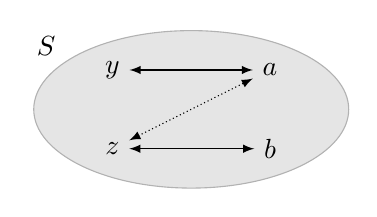
\begin{tikzpicture}[>=latex, scale=1.0]
\def\matchingellipse{(0,0) ellipse (2 and 1)}
\filldraw[fill=gray!20, draw=gray!60]\matchingellipse;
\node[left] at (-1.6,0.8) {$S$};
\node (y) at (-1.0,0.5) {$y$};
\node (a) at (1.0,0.5) {$a$};
\node (z) at (-1.0,-0.5) {$z$};
\node (b) at (1.0,-0.5) {$b$};
\draw[latex -latex] (y) -- (a);
\draw[latex -latex] (z) -- (b);
% \draw[densely dotted, latex-latex] (z) .. controls (-0.4,-1.3) and (0.4,1.3) .. (a);
\draw[densely dotted, latex-latex] (z) -- node[pos=0.5]{\textcolor{red}{\Lightning}} (a);
\end{tikzpicture}
\]

Let \(S\) be a stable matching in which \(y\) is matched with \(a\) (it exists, since \(a\) is a valid partner of \(y\)).
Let \(b\) be the partner of \(z\) in \(S\).
\(z\) has not been rejected/dumped by any valid partner (including \(b\)) at the point when \(y\) is rejected/dumped by \(a\), because the latter is the first such event during \autoref{alg:gale_shapley}.
That means \(z\) has not yet proposed to \(b\) when he proposes to \(a\), so \(z\) prefers \(a\) to \(b\).
Thus \((z,a)\) is an unstable pair in \(S\), contradicting the stability of \(S\).
\end{proof}

It can be proven that the \(M\)-optimal matching produced by \autoref{alg:gale_shapley} is unique and \(W\)-pessimal, i.e., each \(w \in W\) is matched with their worst valid partner.



\subsection{Implementation}

We want to implement \autoref{alg:gale_shapley} in \(O(n^2)\) time.
This means one iteration of the while-loop must take \(O(1)\) time.

\medskip

To that end, we need to be able to answer the question ``Does \(w\) prefer \(m\) to her current partner \(m'\)?'' in \(O(1)\) time!
Let's say that each \(w \in W\) has a preference array \(\texttt{pref}_w = [m_1, \ldots, m_n]\), where \(m_i\) is the \(i\)-th most preferred man for \(w\).
To answer the above question in constant time, we build an inverse preference array \(\texttt{inverse}_w\) in \(O(n)\) time once for each \(w \in W\) as a preprocessing step.

\begin{algorithm}[h]
\caption{Build Inverse Preference Arrays}
\label{alg:build_inverse_preference_arrays}
\begin{algorithmic}[1]
\Require for each \(w \in W\), a preference array \(\texttt{pref}_w\) such that \(\texttt{pref}_w[i]\) gives the \(i\)-th most preferred man for \(w\)
\Ensure for each \(w \in W\), an inverse preference array \(\texttt{inverse}_w\) such that \(\texttt{inverse}_w[m]\) gives the rank of \(m\) in \(w\)'s preference list
\For{each \(w \in W\)}
  \State initialize the array \(\texttt{inverse}_w\) of size \(n\)
  \For{\(i \gets 1 \TO n\)}
    \State \(\texttt{inverse}_w[\texttt{pref}_w[i]] \gets i\) 
  \EndFor
\EndFor
\end{algorithmic}
\end{algorithm}


\subsection{Other Properties}\label{sec:other_properties}

\begin{claim}\label{clm:gale_shapley:women_any_pairing}
Suppose all men use the same preference list \(l: w_1 \succ \cdots \succ w_n\).
If the women know about \(l\), they can force \autoref{alg:gale_shapley} to return any desired pairing \(P\).
\end{claim}

\begin{proof}[Induction]\label{proof:gale_shapley:women_any_pairing}
Consider the desired pairing \(P=\{(w_i,m_i)\}_{i=1}^n\).
Let every woman \(w_i\) submit a {fake} preference list that places \(m_i\) at the very top
(the order of the remaining men is arbitrary).

\begin{enumerate}[partopsep=0em, label=(\roman*)]
\item Base case:
When it is \(m_1\)'s time to propose, he will first propose to \(w_1\), since all men share the list \(l\).
Because \(m_1\) is ranked first by \(w_1\), she accepts and will never dump him (\autoref{obs:gale_shapley:women_only_trade_up}).
So \((w_1,m_1)\) is permanently formed.
\textcolor{Green}{\ding{52}}

\item Induction hypothesis:
Assume for some \(k\ge 2\) that \((w_i,m_i)\) are permanently matched for all \(i<k\). 
\label{proof:gale_shapley:women_any_pairing:induction_hypothesis}

\item Induction step:
Consider \(m_k\).
% By \autoref{obs:gale_shapley:men_propose_in_decreasing_order}, \(m_k\) proposed (in sequence) to \(w_1,w_2,\ldots,w_{k-1}\) before \(w_k\).
% Each \(w_i\) with \(i<k\) rejects \(m_k\), because she is already engaged to her top choice \(m_i\).
Because of \ref{proof:gale_shapley:women_any_pairing:induction_hypothesis}, each \(w_i\) with \(i<k\) is already permanently matched with her top choice \(m_i\) and thus rejected/dumped \(m_k\) at some point.
So \(m_k\) eventually proposes to \(w_k\), who ranks \(m_k\) first and accepts.
By \autoref{obs:gale_shapley:women_only_trade_up}, \(w_k\) never drops \(m_k\), so \((w_k,m_k)\) is permanent.
\textcolor{Green}{\ding{52}}
\end{enumerate}

By induction, all pairs \((w_i,m_i)\) form and remain, so the algorithm returns \(P\).
\end{proof}

\begin{claim}
There is at most one man \(m^* \in M\) such that the matching created by \autoref{alg:gale_shapley} matches \(m^*\) with his last-choice woman \(w^*\).
Moreover, at the moment \(m^*\) is matched with \(w^*\), \autoref{alg:gale_shapley} terminates.
\end{claim}

\begin{proof}
Let \(m^*\) be the first man to propose to his last-choice woman \(w^*\) in \autoref{alg:gale_shapley}.
By \autoref{obs:gale_shapley:men_propose_in_decreasing_order}, he has proposed to every \(w\in W\setminus\{w^*\}\) and been rejected/dumped and by \autoref{obs:gale_shapley:women_only_trade_up}, each such \(w\) is (and stays) engaged. 
Hence exactly \(n-1\) women (and thus \(n-1\) men) are engaged, so \(m^*\) is the unique free man.
If \(w^*\) were engaged, there would be \(n\) engaged men, contradicting that \(m^*\) is free. 
Therefore \(w^*\) is free and accepts \(m^*\), yielding \(n\) engaged pairs and immediate termination.
%Since the algorithm stops here, no second man can ever reach his last choice.
\end{proof}
